\chapter{Analyse et Spécifications des Besoins}
\label{chap:analyse_specifications_besoins}

\section{Introduction}

Ce chapitre vise à explorer en détail les besoins de notre application en matière de conversion de wireframes dessinées à la main en interfaces web fonctionnelles. Nous commencerons par identifier les acteurs impliqués dans le processus, puis nous détaillerons les besoins fonctionnels et non fonctionnels de l'application. Ensuite, nous établirons le backlog du produit, planifierons les sprints à venir et présenterons un diagramme de cas d'utilisation général pour mieux comprendre les interactions entre les utilisateurs et le système.

\section{Spécification des besoins}

\subsection{Identification des acteurs}

Les principaux acteurs impliqués dans notre application sont les suivants :

\textbf{Client (Développeur)} : Le client est l'utilisateur principal de l'application. Il importe une capture scannée d'une wireframe dessinée à la main dans l'application, récupère ensuite le code généré pour validation avec le client avant de poursuivre le processus de développement.

\subsection{Besoins fonctionnels}

Les besoins fonctionnels de notre application comprennent les éléments suivants :

\begin{itemize}
    \item \textbf{Téléchargement des wireframes :} Les utilisateurs doivent pouvoir télécharger facilement les wireframes dessinées à la main dans l'application.
    \item \textbf{Reconnaissance des éléments :} L'application doit être capable de reconnaître les différents éléments présents dans les wireframes, tels que les barres de navigation, les boutons, les images, etc.
    \item \textbf{Génération de code :} Une fois les éléments reconnus, l'application doit générer du code HTML/CSS ou React.js correspondant à la structure des wireframes.
    \item \textbf{Téléchargement du code généré :} Les utilisateurs doivent pouvoir télécharger le code généré pour l'intégrer dans leurs projets de développement.
\end{itemize}

\subsection{Besoins non fonctionnels}

Les besoins non fonctionnels de l'application comprennent les aspects suivants :

\begin{itemize}
    \item \textbf{Performance :} L'application doit être capable de traiter les wireframes de manière efficace, même pour des fichiers volumineux.
    \item \textbf{Sécurité :} Les données téléchargées par les utilisateurs doivent être sécurisées et protégées contre tout accès non autorisé.
    \item \textbf{Compatibilité :} L'application doit être compatible avec différents navigateurs web et dispositifs, afin de garantir une expérience utilisateur cohérente.
    \item \textbf{Convivialité :} L'interface utilisateur de l'application doit être intuitive et facile à utiliser, même pour les utilisateurs novices.
    \item \textbf{Flexibilité :} Les utilisateurs doivent avoir la possibilité de personnaliser certains aspects du code généré en fonction de leurs besoins spécifiques.
    \item \textbf{Extensibilité :} La structure de l'application doit être conçue de manière à permettre l'ajout facile de nouvelles fonctionnalités à l'avenir.
\end{itemize}

\section{Backlog du produit}

Le backlog du produit comprendra une liste priorisée des fonctionnalités à développer pour l'application, en se basant sur les besoins identifiés. Il sera mis à jour régulièrement pour refléter les évolutions du projet et les retours des utilisateurs.

\section{Planification des sprints}

Nous utiliserons la méthodologie SCRUM pour planifier les sprints à venir. Chaque sprint sera consacré à la réalisation d'un ensemble spécifique de fonctionnalités du backlog du produit, avec des objectifs clairement définis et une durée fixe.

\section{Diagramme de cas d'utilisation général}

Le diagramme de cas d'utilisation général représente les interactions entre les différents acteurs et les fonctionnalités de l'application. Il permet de visualiser les scénarios d'utilisation les plus courants et de mieux comprendre le fonctionnement global du système.

\begin{figure}[H]
    \centering
    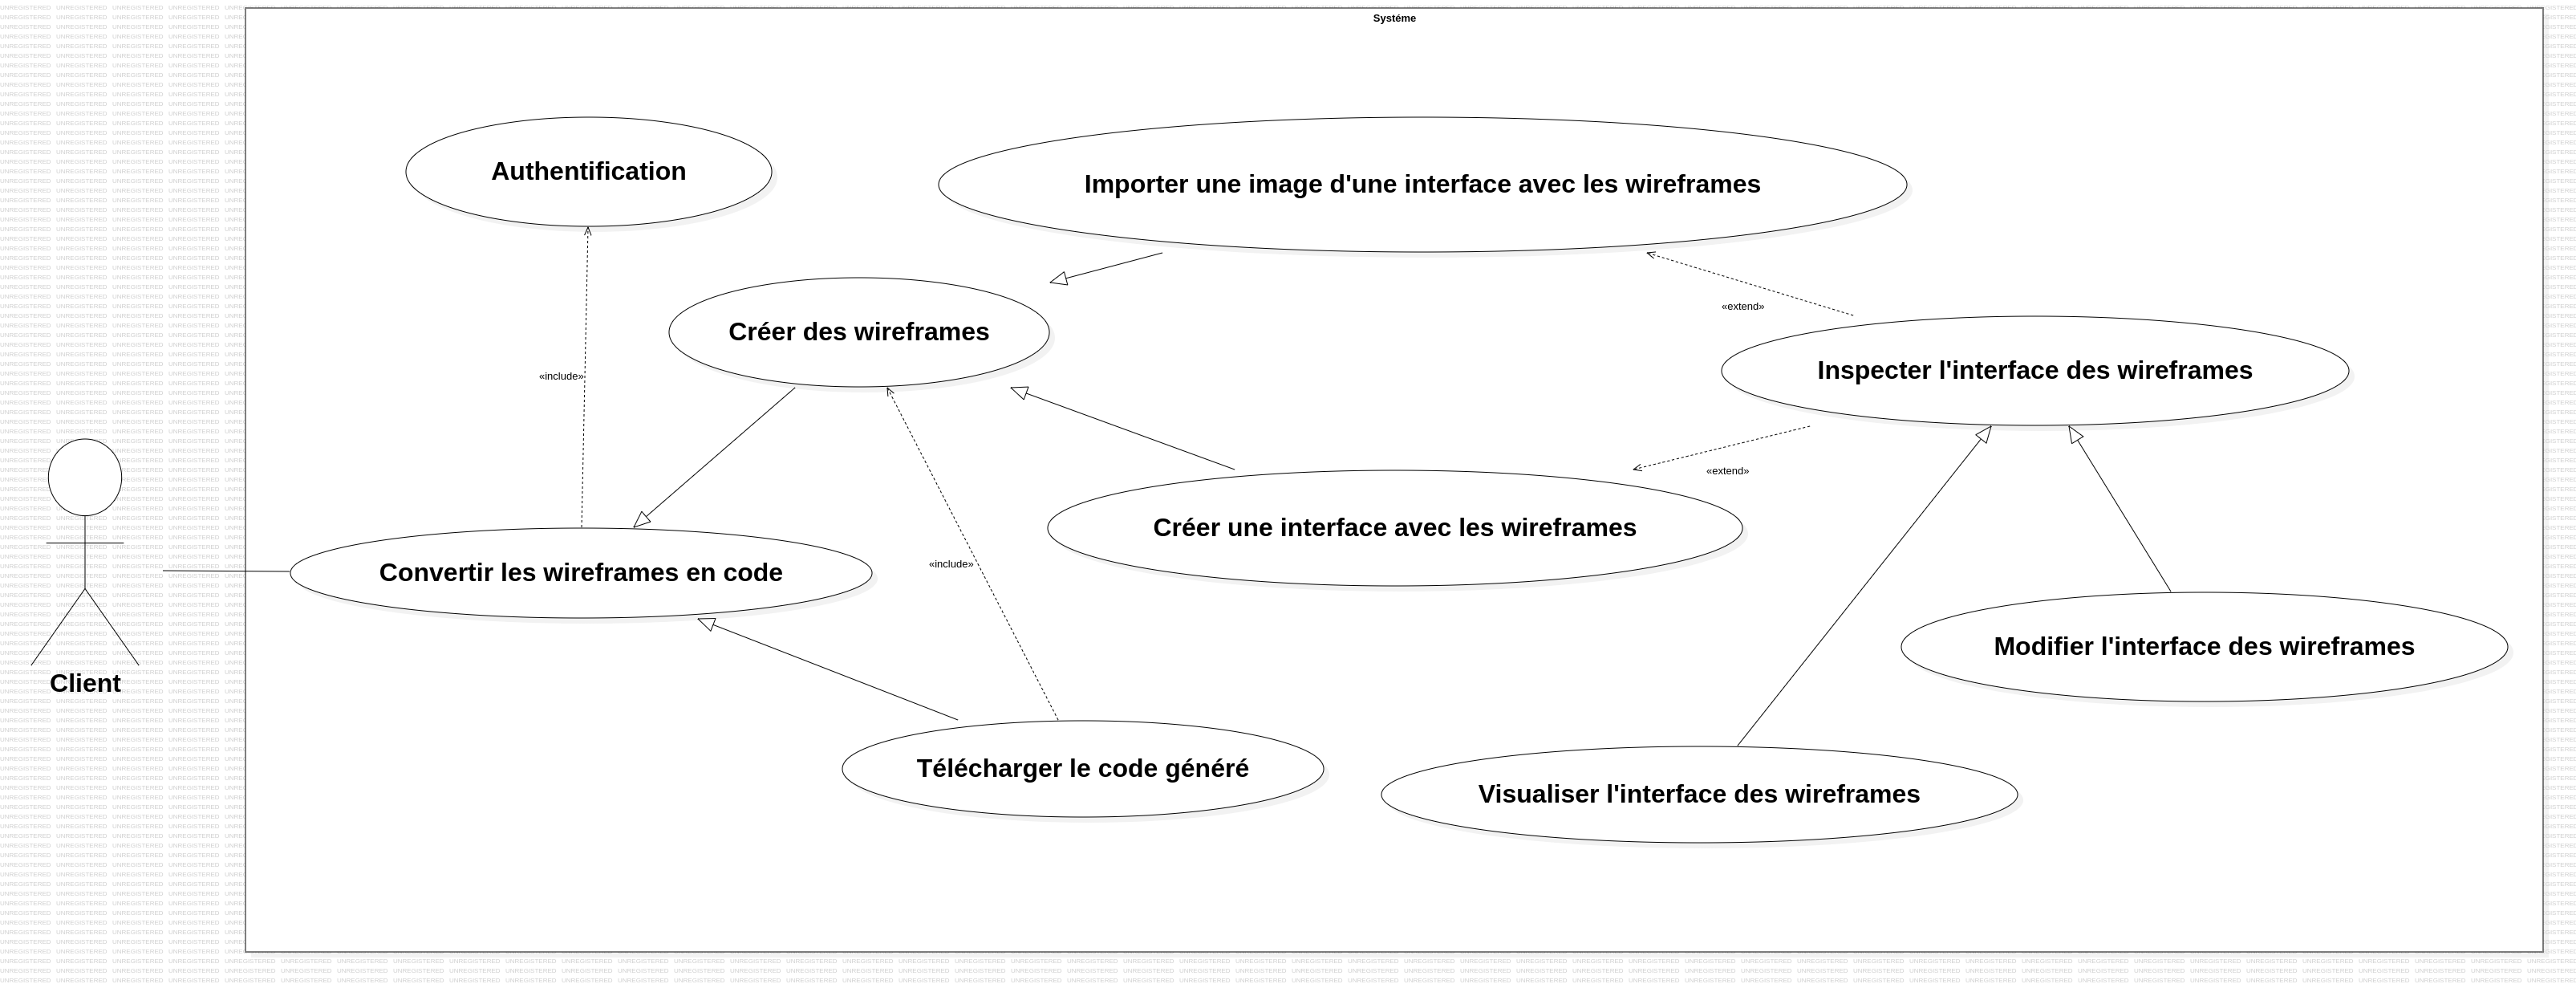
\includegraphics[width=1\linewidth,height=8cm]{images/UseCaseDiagram1.png}
    \caption{Diagramme des cas d'utilisations global}
    \label{fig:diagramme_cas_utilisation}
\end{figure}

\section{Conclusion}

Ce chapitre a permis de définir les spécifications des besoins de notre application, en identifiant les acteurs impliqués, en détaillant les besoins fonctionnels et non fonctionnels, en établissant le backlog du produit, en planifiant les sprints à venir et en présentant un diagramme de cas d'utilisation général. Ces informations jetteront les bases du développement de l'application et guideront nos efforts futurs pour répondre aux attentes et aux exigences des utilisateurs.
